\documentclass[
10pt, % Main document font size
letterpaper, % Paper type, use 'letterpaper' for US Letter paper
oneside, % One page layout (no page indentation)
%twoside, % Two page layout (page indentation for binding and different headers)
headinclude,footinclude, % Extra spacing for the header and footer
BCOR5mm, % Binding correction
]{scrartcl}


\usepackage{mike}
% include image package and the images folder
\usepackage{graphicx}
\graphicspath{ {Diagrams/} }

%----------------------------------------------------------------------------------------
%	TITLE AND AUTHOR(S)
%----------------------------------------------------------------------------------------

\title{\normalfont\spacedallcaps{Remote EJB Setup and Invocation}} % The article title

\author{\spacedlowsmallcaps{Michael Meding* , mikeymeding@gmail.com}} % The article author(s) - author affiliations need to be specified in the AUTHOR AFFILIATIONS block

\date{} % An optional date to appear under the author(s)

%----------------------------------------------------------------------------------------

\begin{document}

\maketitle % Print the title and abstract box

\setcounter{tocdepth}{2} % Set the depth of the table of contents to show sections and subsections only

\tableofcontents % Print the contents section

\thispagestyle{empty} % Removes page numbering from the first page

%----------------------------------------------------------------------------------------
%	ARTICLE CONTENTS
%----------------------------------------------------------------------------------------
 
\section*{Abstract}
Write about how this article is structured and what will and will not be covered and why. 
Discuss the diagram below. Exclusively wildfly setup
 
~\newline
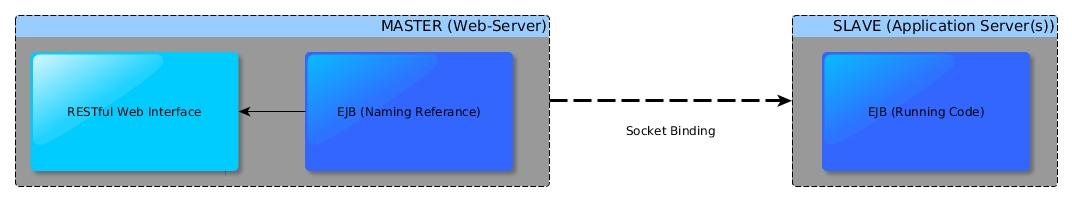
\includegraphics[width=13.75cm]{EJBDiagram} % FLOWCHART

%------------------------------------------------

\section{Setting Up Wildfly}

%------------------------------------------------

\paragraph{} Explain how the following sub sections have to do with setting up the standalone-full.xml

%------------------------------------------------

\subsection{secret}

%------------------------------------------------

\paragraph{XML}~
%Code Snippet
\lstsetxml % bring in xml highlight settings
\begin{lstlisting}[language=XML]

add some lovely code snippets from standalone here

\end{lstlisting}

%------------------------------------------------

\subsection{remote-mallorca}

%------------------------------------------------

\paragraph{XML}~
%Code Snippet
\lstsetxml % bring in xml highlight settings
\begin{lstlisting}[language=XML]

add some lovely code snippets from standalone here


\end{lstlisting}

%------------------------------------------------

\subsection{outbound-socket-binding}

%------------------------------------------------

\paragraph{XML}~
%Code Snippet
\lstsetxml % bring in xml highlight settings
\begin{lstlisting}[language=XML]

add some lovely code snippets from standalone here

\end{lstlisting}




%------------------------------------------------

\section{Master Side Application Code}

%------------------------------------------------

%------------------------------------------------

\subsection{@EJB}

%------------------------------------------------

\paragraph{JAVA}~
%Code Snippet
\lstsetjava % brings in the java code highlight parameters
\begin{lstlisting}[language=Java]
// some java code here
public class JavaAwesome{
	private static String WOW = "MUCH JAVA";
}
\end{lstlisting}

%------------------------------------------------

\subsection{@PostConstruct}

%------------------------------------------------

\paragraph{JAVA}~
%Code Snippet
\lstsetjava % brings in the java code highlight parameters
\begin{lstlisting}[language=Java]
// some java code here
public class JavaAwesome{
	private static String WOW = "MUCH JAVA";
}
\end{lstlisting}


%------------------------------------------------

\subsection{jboss-ejb-client.xml}

%------------------------------------------------

\paragraph{XML}~
%Code Snippet
\lstsetxml % bring in xml highlight settings
\begin{lstlisting}[language=XML]

add some lovely code snippets from standalone here


\end{lstlisting}




%------------------------------------------------

\section{Slave Side Code Deployment}

%------------------------------------------------

%------------------------------------------------

\subsection{standalone-full.xml}

%------------------------------------------------

\paragraph{XML}~
%Code Snippet
\lstsetxml % bring in xml highlight settings
\begin{lstlisting}[language=XML]

add some lovely code snippets from standalone here

\end{lstlisting}

%------------------------------------------------

\subsection{Please Note!}

%------------------------------------------------

% explain here about needing a correct user to gain access to EJB
% also expain about .jar/.ear



\end{document}
